\scanpage{8}
\uline{Theorem 1} Let $\pi$ be a discrete group, $E$ a $\pi$-principal covering of a space $B$.
Consider for \inserted{every} space $X$ the map
\[
\operatorname{hot}(X,B)\xrightarrow{h_X}H^1(X,\pi)
\quad\bigl(\overset{\mathrm{df}}=\text{isomorphism classes of principal $\pi$-coverings of $X$}\bigr)
\]
\figure{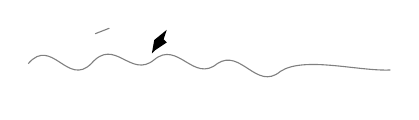
\begin{tikzpicture}
\draw[gray] (.85,.38)--(1.03,.45);
\fill (1.57,.13)--(1.6,.3)--(1.76,.43)--(1.72,.31)--(1.76,.27)--(1.61,.17)--cycle;
\draw[gray] (0,0) .. controls (.3,.35) and (.5,-.3) .. (.8,0)
.. controls (1.1,.35) and (1.3,-.2) .. (1.6,.05)
.. controls (1.9,.3) and (2.1,-.25) .. (2.4,0)
.. controls (2.7,.2) and (2.9,-.35) .. (3.2,-.1)
.. controls (3.5,.1) and (4.2,-.1) .. (4.6,-.08);
\end{tikzpicture}}
functorial in $X$.
\figure{
\begin{tikzpicture}\draw (0,.1) .. controls (.12,-.08) and (.53,-.1) .. (.38,.1) -- (.12,.25) .. controls (.35,.13) and (.63,.03) .. (.48,.36) -- (.4,.55) .. controls (.43,.64) and (.7,.64) .. (.78,.78);\end{tikzpicture}}

Equivalent conditions

1) $h$ is an isomorphism of functors,

\hspace*{2em}i.e. \deleted{\unsure{in}}\inserted{bi}jective for $\forall\ X$

(One then says that $(E,B,\pi)$ is a universal $\pi$-covering, $B$ is called ``the classifying space'' for $\pi$)

2) $E$ is contractible

\mspage{7}
